\documentclass[11pt, reqno]{amsart}

\usepackage[utf8]{inputenc}
\usepackage[T2A]{fontenc}
\usepackage[english,ukrainian]{babel}

\usepackage{imnanu}  % main style file

\usepackage{amssymb}
\usepackage{graphicx}
\usepackage{xcolor}
\usepackage[all]{xy}
\usepackage{hyperref}
\hypersetup{hidelinks, hypertexnames=false} %% <-- no colors for links
% \hypersetup{
% 	hypertexnames=false,
% 	colorlinks,
% 	linkcolor={red!50!black},
% 	citecolor={blue!50!black},
% 	urlcolor={blue!80!black}
% }

%% if you need to change parameters
% \SET{\Year}{2021}
% \SET{\Volume}{12}
% \SET{\Number}{5}

\begin{document}
%%%%%%%%%%%%%%%%%%%%%%%%%%%%%%%%%%%%%%%%%%%%%%%%%
%!!!!!! do not change this line - it will print the correct number of the first page
\label{first_page:\thearticlesnum}
%%%%%%%%%%%%%%%%%%%%%%%%%%%%%%%%%%%%%%%%%%%%%%%%%

%%%%%%%%%% PRINT INFORMATION ABOUT AUTHORS

%------ uncomment paper language
\setlanguage{ukrainian}
% \selectlanguage{english}


%------ information about each author

\author{О.~С.~Лимарченко}
\address{Київський національний університет імені Тараса Шевченка}
\email{olelim2010@yahoo.com}
\orcid{0000-0002-2068-8987}


\title[Аналітичної механіки суцільного середовища]{Розширені можливості аналітичної механіки суцільного середовища}

%------ abstracts
\abstract{english}{
Advanced potentials of analytical mechanics of continuum medium and sources promoted the appearance, development and high achievements of this direction of research namely in Ukraine are under discussion. We traced connections of this direction with D.O. Grave and his follower M.~O.~Kilchevsky. We shortly state and show by examples new elements of this approach and its advantages. It is shown that similar research are developed now in Ukraine.}

\abstract{ukrainian}{
Обговорюються розширені можливості аналітичної механіки суцільного середовища і джерела, які сприяли виникненню, розвитку і високим досягненням такого напрямку досліджень саме в Україні. Відстежуються зв'язки цього напрямку досліджень з Д.~О.~Ґраве і його учнем М.~О.~Кільчевським. Скорочено викладено і проілюстровано на ряді прикладів нові елементи такого підходу і його переваги. Показано, що подібні дослідження і дотепер розвиваються саме в Україні.
}


\keywords{Ґраве, Кільчевський, принцип Гамільтона, в’язі, коливання рідини з вільною поверхнею}
\udc{532.595}
\msc{70H25; 01A72}
%% DOI of the current paper
% \doi{}

\maketitle
%\begin{document}



\section*{Вступ}
При викладенні теоретичної механіки та деяких розділів фізики переважно аналітичній механіці відводиться роль деякого апарата, який по аналогії з другим законом Ньютона дозволяє одержати математичну модель системи у вигляді диференціальних рівнянь. Специфічною особливістю методів аналітичної механіки є те, що на простих прикладах усі переваги такого підходу не розкриваються, проте надмірна громіздкість і складність мають місце. Оскільки у звичайних вишівських курсах обмежуються саме такими прикладами, то загальне враження від методів аналітичної механіки залишається таке, що цей підхід не є конструктивним, а є лише методичним. В більшості вишів методи аналітичної механіки суцільних середовищ взагалі не вивчаються. Коли М.~О.~Кільчевському в різних обговореннях щодо методів аналітичної механіки казали про подібну обмеженість аналітичної механіки, то він часто вживав відомий афоризм Д.~І.~Менделєєва "Нафта не паливо, опалювати можна й асигнаціями". В роботі буде дано опис розширених можливостей методів аналітичної механіки суцільних середовищ в теоретичному і конструктивному напрямках.


\section{Микола Олександрович Кільчевський, 1909--1979}
Мені пощастило бути аспірантом академіка АН УРСР Миколи Олександровича Кільчевського. Під час навчання в Київському університеті він мені не читав лекції, але за підказкою досвідчених доцентів кафедри теоретичної механіки, на якій я проходив спеціалізацію, я познайомився з М.~О.~Кільчевським і після коротких обговорень і уточнень теми дипломної роботи саме під його керівництвом я провів дослідження задачі про імпульсне збурення руху стисливого газу в циліндричній камері. В ході двох зустрічей з ним я одержав пропозицію вступити до нього в аспірантуру. Для мене було дивним, але щонайменше п'ять осіб з університету і з Інституту механіки АН УРСР застерігало мене від вступу в аспірантуру саме до М.~О.~Кільчевського. Але я пообіцяв, перейшов на роботу в Інститут механіки АН УРСР, вступив до аспірантури, достроково захистив кандидатську дисертацію і ніколи не шкодував що пішов працювати саме з М.~О.~Кільчевським. Спочатку М.~О.~Кільчевський прохолодно до мене відносився, проте ''проекзаменувавши'' мене по ряду питань (наукових і загальних) став відноситися більш приязно. На моє прохання визначити мені тему дисертації він відповів, що дурням визначає теми сам, а розумні це мають робити самостійно. Через тиждень я запропонував тему, яку він схвалив, хоча відмітив, що очікував інший напрямок. Так я став займатися задачами динаміки конструкцій з рідиною з вільною поверхнею, причому з перших кроків в сумісній і в нелінійній постановці. Нашим бесідам не лише за темою моєї роботи сприяло те, що Б.~Є.~Патон, який сам слухав лекції М.~О.~Кільчевського, направляв Миколі Олександровичу на експертизу проєкти всіх ''вічних двигунів'' і ''безінерційних рушіїв'', які надходили до Президії АН УРСР. Зазвичай М.~О.~Кільчевский давав по черзі такі проєкти своїм аспірантам, а потім уважно слухав підготовлені версії відгуків аспірантів, уточнював їх і за підписами академіка та аспіранта цей відгук повертався до Президії АН УРСР. Поступово я ''набив руку'' і майже всі відгуки писав сам. При обговоренні таких проєктів дрібниць не було. Я підлягав жорсткій критиці як за манери побудови речень на наукові теми, так і за стиль написання. За що я безмежно вдячний М.~О.~Кільчевському: стиль викладення матеріалу він мені прищепив. Часто також М.~О.~Кільчевський доручав мені готувати відгуки на автореферати дисертацій.

М.~О.~Кільчевський не був би собою якби під час різних обговорень таких проєктів і моїх досліджень він би не робив посилання на свій попередній досвід, своїх колег і свою наукову школу. З величезною вдячністю він згадував Д.~О.~Ґраве, якого вважав своїм керівником. Згадуючи про Д.~О.~Ґраве Микола Олександрович завжди відзначав його наукову і культурну енциклопедичність. Він був науковим експертом по широкому колу питань, завжди звертав увагу на культурний рівень співробітників. Учениця Д.~О.~Ґраве Т.~В.~Путята розповідала що на квартирі Д.~О.~Ґраве відбувалися зустрічі аспірантів і співробітників, на яких обов'язковою складовою було виконання музичних партій на фортеп'яно. Більш того, Д.~О.~Ґраве міг сказати приблизно наступне: ''Ваше виконання цього твору свідчить, що сьогодні ви не готові до наукової консультації''. Тобто він через музику бачив духовний стан і схильність до творчості. Він вчив всіх добрим манерам, новинкам культури та новим поглядам в науці. М.~О.~Кільчевський розповідав, що Д.~О.~Ґраве все життя відточував свою лекційну майстерність. З посмішкою він розповідав про один методичний винахід Д.~О.~Ґраве. Щоб наголосити, що деякі величини в математиці й механіці не є малими, він малював диференціал і деякі вектори ледь не на всю дошку, при цьому він сильно вдаряв крейдою в точці початку вектора, а потім через декілька кроків вздовж дошки завершував новим ударом по дошці кінець вектора. Тому, коли інколи було чутно значний шум, то всі з посмішкою казали, що турбуватися не треба, просто Д.~О.~Ґраве дійшов до зображення диференціала. Д.~О.~Ґраве казав, що на лекції викладач має бути й знавцем, і педагогом, і актором одночасно.


На початку минулого століття в механіці було два потужних ''стрибка'': первинне формування асимптотичних методів нелінійної механіки та перегляд деяких положень плідної на той час теорії оболонок. Ще А.~Айнштайн вказав на певну суперечність теорії оболонок, яке було пов'язане з тим, що класичні методи теорії оболонок приводили до еліптичних крайових задач з нескінченими швидкостями поширення збурень, а фізично вірогідними мали б бути гіперболічні постановки задач, яким притаманні скінчені швидкості поширення збурень. Відомо про контакти Д.~О.~Ґраве з А.~Aйнштейном з питань теорії відносності (я не бачив офіційного підтвердження цього, проте були згадки про це) і не виключено, що й ширше коло питань обговорювалося ними. В Київському політехнічному інституті в ті часи працював С.~П.~Тимошенко, який в контакті з П.С. Еренфестом створив теорію балок і оболонок, яка вже призводила до систем рівнянь гіперболічного типу. Проте ця теорія, яка включала інерцію зсувних рухів перерізів пружних тіл, не виглядала строго математично обґрунтованою. З точки зору М.~О.~Кільчевського це була теорія, що включала додаткову механічну гіпотезу, яка не виглядала бездоганно обґрунтованою. Тому на початку 30-х років минулого століття М.~О.~Кільчевський і незалежно І.~М.~Векуа почали створення нових математично обґрунтованих теорій оболонок. Як підсумок такої успішної роботи М.~О.~Кільчевський в 1939 році захистив докторську дисертацію. Через смерть Д.~О.~Ґраве науковим консультантом цієї роботи виступив І.~Я.~Штаєрман. Пізніше М.~О.~Кільчевський був залучений до виконання різних оборонних замовлень, а потім зосередив свою увагу на задачі про динамічне контактне стискання твердих тіл, за що був нагороджений Державною премією УРСР, а потім послідовно був обраний членом-кореспондентом АН УРСР і академіком АН УРСР. Крім того М.~О.~Кільчевський був обраний до складу бюро Національного Комітету СРСР з теоретичної та прикладної механіки, що автоматично включало його до складу запрошених гостей на засідання Академії наук СРСР, тому він був у курсі всіх основних новин наукового життя і мав численні контакти з колегами не лише з України.

М.~О.~Кільчевському належить видатний двотомний підручник з теоретичної механіки. Ця книга є не лише книгою з теоретичної механіки, а є ще й видатною роботою з філософії природничих наук. В 90-ті роки я познайомився з академіком НАН України М.~В.~Поповичем, відомим філософом, політиком. Він розповідав, що у свої молоді роки читав лекції з філософії природознавства студентам, інженерам. Одного разу після лекції він одержав від досвідченого слухача значну порцію критики та настанову, що йому слід прочитати підручник з теоретичної механіки М.~О.~Кільчевського, щоб впорядкувати свої знання. М.В. Попович розповідав мені, що він був в захваті від цього підручника і навіть не очікував що одержить таке джерело для подальшого розуміння проблем. Що вже казати про значення цього підручника для фахівців-механіків. Характерною рисою цього підручника є викладення механіки як складової частини природознавства в цілому і математики, а не просто інженерії, що безумовно було зроблено під впливом робіт Д.~О.~Ґраве \cite{G081},\cite{G30}.

Надалі М.~О.~Кільчевський приділив основну увагу розвиненню методів аналітичної механіки континуальних систем. Він зі співавторами випустив три монографії ''Основы аналитической механики оболочек'', ''Лекции по аналитической механике оболочек'', ''Аналитическая механика континуальных систем''. Роки, стан здоров'я брали своє і свою публікаційну активність він знизив. Проте мені пощастило під час чисельних зустрічей з М.~О.~Кільчевським обговорити багато наукових і науково-методичних проблем аналітичної механіки та, я думаю, вірно зрозуміти його ставлення до багатьох етапів цієї теорії, основні етапи якої я надалі спробую донести до читачів. Звичайно ці положення значною мірою переломлені через мій досвід і моє засвоєння (сподіваюся не хибне) цих проблем.

\section{Основні переваги методів аналітичної механіки в задачах руху суцільних середовищ}
Викладення матеріалу в цьому розділі проводиться на основі ідей і формулювань М.~О.~Кільчевського, але в моїй інтерпретації й з моїми осучасненими уточненнями та доповненнями й переважно не на основі статей, книжок, а на основі бесід під час консультацій в період мого навчання в аспірантурі. Тому за всі неточності та недоліки беру відповідальність на себе.

Варіаційні принципи механіки бувають різними. В основному їх поділяють на дві групи: диференціальні та інтегральні принципи. Між собою ці принципи поділяються як формою функціоналів, так і вибором рухів порівняння. Традиційно випадки, коли не існує функціоналів, а є лише варіаційні співвідношення, називають варіаційними принципами умовно.
М.~О.~Кільчевський особливу глибину змісту бачив саме у виборі рухів порівняння. Багаторічні дослідження в галузі варіаційних принципів свідчать про те, що найчастіше використовується варіаційний принцип Гамільтона -- Остроградського, який до того ж є найбільш універсальним і конструктивним в плані одержання прикладних результатів. Тому надалі в цій роботі будемо орієнтуватися на цей варіант варіаційного принципу. Насамперед слід визначити співвідношення між системою законів Ньютона і варіаційними принципами механіки. Значна частина дослідників відводять варіаційному принципу  Гамільтона -- Остроградського підпорядкований статус, ставлячи на перше місце закони Ньютона. В більшості підручників з механіки доведенням коректності варіаційного принципу вважається те, що варіаційний принцип Гамільтона -- Остроградського можна вивести з рівнянь Ньютона (коректніше з диференціального варіаційного принципу Даламбера -- Лагранжа). Проте ще з часів П.~Мопертюі має право на життя й інша думка, що в побудові основних законів механіки варіаційні принципи та закони Ньютона є еквівалентними \cite{Pol}.

Найбільш повно основні переваги варіаційних принципів механіки були викладені в \cite{Pol}. В основному вони зводяться до таких властивостей.

1. Інваріантність формулювань варіаційних принципів відносно геометрії вивчаємих областей, що створює значні переваги при дослідженні задач з неканонічними формами областей.

2. Використання варіаційних принципів в механіці суцільних середовищ забезпечує коректність постановки крайових задач. При цьому кінематичні граничні умови є неодмінною складовою частиною реалізації варіаційних принципів і мають бути задовільнені заздалегідь, а динамічні граничні умови є природними для варіаційних формулювань задач. Тому форма і кількість граничних умов є невіддільною складовою реалізації варіаційного апарату. Більш того, цей апарат не буде працювати для некоректно поставлених задач, що відразу викликає потребу в ревізії вихідної постановки проблеми і, більш того, вказує на місце, де ця ревізія потрібна.

3. Варіаційні принципи природним чином описують рух всіх компонент системи та її взаємодію на основі властивості адитивності енергетичних характеристик. Варіювання призводить до одержання в аналітичному вигляді сил взаємодії між компонентами. Адитивність енергетичних характеристик дозволяє поєднувати механічні системи з підсистемами немеханічної природи, наприклад, з тепловими явищами, електромагнітними тощо.

4. Основні складності методичного типу, які потребують значної уваги при застосуванні методів розв'язання заснованих на постановках задач в диференціальному вигляді, стають схованими при формальній реалізації алгоритмів варіаційних методів і долаються на етапі формального виконання техніки варіювання.

Існує також розширення варіаційного принципу на релятивістські системи, проте тут ми не будемо аналізувати цю тему. Зазвичай вважалося що саме цим вичерпувалися можливості варіаційних принципів. М.~О.~Кільчевський наголошував, що головним у варіаційних принципах механіки є не саме екстремальне співвідношення, а вибір варіацій змінних, рухів порівняння. Нагадаємо, що в варіаційному принципі Гамільтона -- Остроградського варіації змінних визначають рухи порівняння та обираються як можливі переміщення додатково наділені вимогою ізохронності. Отже, в підсумку рухи порівняння визначаються як

1) малі переміщення точок системи,

2) які в заданий момент часу (час зупинено)

3) задовільняють кінематичним обмеженням задачі (в'язям, а у випадку суцільного середовища ще й іншим обмеженням) і є

4) ізохронними.

Отже, пункт 1) визначає техніку варіювання функціонала, пункти 2) і 3) визначають характер задовільнення в’язей, а пункт 4) дозволяє специфікувати екстремалі. Головною проблемою є звичайно задовільнення в’язей. М.~О.~Кільчевський взагалі вважав, що ''аналітична механіка є наукою про в’язі''.  На основі аналізу в’язей і їх порівняння згідно з його підходом можна зробити багато корисних висновків про поведінку системи.

Новим елементом, який був відзначений у бесідах із М.~О.~Кільчевським було визначення міри обмеження руху системи, яке накладається в'язями. Передумовою є відома теорема \cite{Gan} про збільшення частот коливань при накладанні в'язей. Покажемо хід такого аналізу на прикладі руху резервуара з рідиною. Відомо, що сумісний рух резервуара з рідиною з вільною поверхнею описується достатньо складною моделлю \cite{Limbo}, проте у випадку задачі про визначення частот задача значно спрощується.
Система резервуар~-- рідина при поступальному і кутовому рухах тіла--носія в режимі сумісного руху складових системи в рамках лінійної моделі з утриманням в рівняннях лише першої антисиметричної форми коливань рідини описується такою математичною моделлю.
\begin{eqnarray}\label{1}
   &&\ddot{a_1} +\frac{1}{\alpha_1^v} \ddot{\varepsilon_x} B^1_{1x} +\frac{1}{\alpha_1^v} \ddot{\alpha_2} E^{1*}_{11} +\omega_1^2 a_1 =0;\\
   &&\frac{\rho}{M_r+M_l} \ddot{a_1} B^1_{1x} +\ddot{\varepsilon_x} +\frac{\rho}{M_r+M_l}\ddot{\alpha_2}F_2^1 =0; \nonumber\\
   &&\ddot{a_1} E^{1*}_{11} + 2 \ddot{\varepsilon_x}  F_2^1 \!+ 2 \ddot{\alpha_2} \bigg (\frac{1}{\rho} J_{res}^{22}+E_{11}^2 \bigg )\!\!  +\nonumber\\
   &&\alpha_2 \frac{2g}{\rho} \bigg [ M_r \bigg (l+\frac{H}{4} \bigg) \bigg ]\!\! +M_l \bigg (l+\frac{H}{2} \bigg ) \bigg ]\! \! =0.\nonumber
\end{eqnarray}

Тут $a_1$ амплітуда збудження коливань рідини за першою антисиметричною формою, $\varepsilon_x$ і $\alpha_2$ --- параметри поступального і кутового руху резервуара. Ці параметри є незалежною сукупністю параметрів, які повністю характеризують рух системи. В рівняннях також використано такі позначення $\rho$~--- густина рідини, $g$ --- прискорення вільного падіння, $H$~---
рівень заповнення, $M_r$ і $M_{\rm l}$ --- маса резервуара і рідини, $h_{\rm l}$ і $h_r$ --- зміщення центрів ваги рідини і резервуара відносно площини незбуреної
вільної поверхні, $I_{\rm res}^{ij}$ --- тензор інерції резервуара, визначений відносно полюса, стосовно якого описується обертання резервуара. Індексні коефіцієнти є мірами зв'язаності руху рідини в резервуарі із поступальним і кутовим рухом (вони докладно проаналізовані в \cite{Limbo}).

Розглянемо дві задачі. Нехай резервуар не рухається. В цьому випадку друге і третє рівняння системи \eqref{1} виключаються, а з першого рівняння визначається частота коливань рідини
\begin{eqnarray*}
   &&\omega_0 =\sqrt{\frac {\kappa_1 g}{R} \tanh \frac{\kappa_1 H}{R}}.
\end{eqnarray*}
Розглянемо другу задачу. Нехай тепер резервуар може здійснювати рух в горизонтальному напрямку. Що відбулося з точки зору аналізу в'язей? Фактично в'язь, яка обмежувала поступальний рух, знята. Виходить, що частота має зменшитися. Проте, визначення частоти сумісних коливань системи на основі рівнянь сумісного руху призводить до такої залежності
\begin{eqnarray*}
   &&\omega^2=\frac{\omega_0^2}{1- \displaystyle \frac{\rho (B_{1x}^1)^2}{\alpha_1^x (M_l+M_r)}}.
\end{eqnarray*}
Вираз у знаменнику менший за одиницю, оскільки всі змінні додатні та, беручи до уваги що знаменник більше за нуль, виходить, що частота неочікувано збільшилася. На основі підходу аналітичної механіки та властивостей в’язей це могло відбутися лише внаслідок накладання нових в’язей. Дійсно, після зняття обмеження на поступальний рух резервуара, друге рівняння системи можна проінтегрувати та з нього одержується фактично закон збереження положення центру мас системи (це випливає також з теореми про рух центру мас системи). Таким чином ми з'ясували що з'явилася нова в'язь, яка до того ж призвела до збільшення частоти (цю в'язь можна одержати просто безпосереднім інтегруванням другого рівняння за часом). І тут висновок, який в літературі відсутній: обмеження на рух, обумовленому в'язями при закріпленні резервуара, є меншими, ніж обмеження, які накладає в'язь, що визначає незмінність положення центру мас системи. Фактично в цьому алгоритмі схований метод побудови рейтингу в’язей за мірою їхнього впливу на обмеження рухів точок системи. В ході таких обговорень М.~О.~Кільчеський ще відзначав, що наслідки багатьох гіпотез, які додатково приймаються для спрощення постановок задач, можна проаналізувати до розв'язання задачі з позицій аналізу в'язі. Треба відзначити, що кінематичні обмеження в задачах механіки суцільного середовища можуть приймати незвичні форми в порівнянні із задачами механіки дискретних систем. Наприклад, умова нерозривності (вимога суцільності руху рідини) для випадку потенціального руху ідеальної нестисливої рідини набуває вигляду $\Delta \varphi =0$ і стає для задачі течії рідини старшим диференціальним оператором. До кінематичних обмежень слід також відносити умови збереження об'єму рідини та умови розв'язуваності крайових задач, які теж набувають незвичних форм. Проте надалі такі умови не випливають з варіаційного принципу Гамільтона -- Остроградського (не є природними) і тому мають бути задовільнені на рівні кінематичних в’язей до розв'язання варіаційної задачі.

Другий принциповий момент полягає в оцінюванні потенціальних можливостей варіаційних принципів в конструктивному напрямку. За часів М.~О.~Кільчевського варіаційні принципи використовувалися лише для доведення їхньої еквівалентності постановкам задач виведених на основі законів Ньютона або для виведення математичної моделі системи. Найчастіше після одержання математичної моделі задачі починалося застосування різних спрощувальних гіпотез і різних методів побудови розв'язку. Однією з проблем було і те, що в складних задачах механіки, які описували сумісний рух декількох компонент системи, одержувалася математична модель неоднорідної структури, наприклад, зв'язані системи диференціальних рівнянь в частинних і повних похідних, рівняння руху рідини та пружного тіла в ейлерових і лагранжевих змінних (для яких по-різному задаються граничні умови).

Принциповою пропозицією, яка випливала зі спілкування з М.~О.~Кільчевським, було безпосереднє застосування різних методів розв'язання і гіпотез спрощення до варіаційного формулювання задачі. В більшості задач це приводило до одержання математичної моделі однорідної структури у вигляді системи звичайних диференціальних рівнянь відносно амплітудних параметрів руху складових механічної системи. Мало того, як правило значно спрощувалося виділення незалежних варіацій, а в більшості випадків вдавалося побудувати функцію Лагранжа відносно амплітудних параметрів і потім одержати математичну модель на основі диференціальних рівнянь Лагранжа другого роду. І тут в нагоді був метод Канторовича \cite{Kan}, згідно з яким для задач механіки математично обґрунтовано вдається ввести представлення розв'язку задачі з відокремленими амплітудними параметрами. Цікаво що в другій половині 90-х років з'явився метод Курхенена -- Леві, в якому були використані подібні ідеї, хоча ми з М.~О.~Кільчевським обговорювали такі способи в другій половині 70-х, а в 1979 я захистив кандидатську дисертацію з використанням цього методу.

Для більш глибокого розуміння нововведень представимо дві схеми використання варіаційних принципів механіки. Умовно їх назвемо класична схема і модифікована схема.

{\it Класична схема}. При задовільненні всіх кінематичних обмежень задачі будується функція Лагранжа для механічної системи. При проведенні процедури виділення незалежних варіацій на виході одержуються рівняння руху системи, динамічні граничні умови, сили взаємодії між складовими компонентами системи в аналітичному вигляді. В залежності від складу компонент системи, що досліджується, одержана математична модель може мати неоднорідну математичну структуру. Звернемо увагу, що конструктивна складова в плані наближення до розв'язання системи рівнянь в принципі відсутня.

{\it Модифікована схема}. При задовільненні всіх кінематичних обмежень задачі будується функція Лагранжа для механічної системи. Форма шуканого розв’язку спрощується на основі різних ідей розділення рухів, до яких входять частотне і амплітудне розділення рухів (асимптотичні методи нелінійної механіки), просторове розділення рухів (метод Канторовича, інші  варіаційні методи математичної фізики в тому числі і методи поточкової дискретизації, наприклад, метод скінчених елементів, масштабне розділення рухів на основі методу вейвлетів), використання гіпотез, емпіричних і експериментальних співвідношень. Важливою рисою використання методів розв'язання на етапі до вживання техніки варіювання є властивість вперше відмічена Л.А. Коздобою \cite{Koz}, яка полягає в тому, що всі наближення, що використовуються в рамках реалізації варіаційного принципу Гамільтона -- Остроградського набувають властивостей ізоенергетичності. Тобто на цьому етапі використання наближень не порушує законів збереження енергії. Вживання таких методів у відриві від варіаційного принципу вже не має таких властивостей. При проведенні процедури виділення незалежних варіацій або при одержанні рівнянь на основі перетвореної функції Лагранжа на виході одержуються рівняння руху системи, які задовільняють динамічним граничним умовам, сили взаємодії між складовими компонентами системи в аналітичному вигляді, виражені в амплітудних параметрах. Одержана модель є системою звичайних диференціальних рівнянь (має однорідну математичну структуру). Кількість рівнянь моделі дорівнює кількості ступенів вільності механічної системи, тобто з точки зору розмірності така модель є мінімальною. Одержана система рівнянь просто зводиться до форми Коші, що створює передумови для подальшого використання якісних методів диференціальних рівнянь і методів чисельного інтегрування.

Саме такий підхід був основою для дослідження нелінійних коливань рідини з вільною поверхнею в сумісній постановці задачі, що дозволило вперше розв'язати задачі про рух систем при кутовому русі конструкції--носія, рух рідини в резервуарах різної геометричної форми, параметричні коливання резервуарів з рідиною, задачі керування рухом конструкцій з рідиною, динаміку трубопроводів з рідиною, що тече \cite{Limbo,Kon,Lkib,LS}.

Зараз варіаційні методи механіки активно використовуються в різних розділах механіки. Тенденція така, що чим складніша задача і чим більше в цій задачі складових (часто навіть
немеханічної природи), тим частіше використовуються варіаційні принципи. Слід відзначити також, що традиційно українські вчені частіше використовують варіаційні принципи механіки в порівнянні з вченими інших країн. Наприклад, в Інституті математики НАН України М.~О.~Луковський і О.~М.~Тимоха активно розвивають варіаційні методи дослідження задач механіки рідини з вільною поверхнею на основі варіаційного принципу Бейтмена, а раніше співробітники цієї школи активно використовували варіаційні методи для дослідження задач про визначення частот і форм коливань рідини, включаючи задачі про гідропружні коливання. Ризикну стверджувати, що ніде у світі так плідно і конструктивно варіаційні принципи механіки не вживаються. Найбільш ймовірно що саме вплив Д.~О.~Ґраве і М.~О.~Кільчевського і їх численних учнів-викладачів обумовив своєрідне сприйняття українськими вченими варіаційних принципів механіки.


\section{Коливання рідини з вільною поверхнею в резервуарах нециліндричної форми}
Одним із яскравих прикладів застосування варіаційного принципу Гамільтона -- Остроградського з поглибленим аналізом кінематичних обмежень задачі є задача про нелінійні коливання ідеальної однорідної рідини в резервуарі у формі тіла обертання. Ця задача є актуальною в теоретичному і практичному сенсі й, попри давнє обговорення способів її розв'язання, існує мало практичних алгоритмів реалізації таких підходів. Звичайно це пов'язане із нециліндричністю області, яку займає рідина, і тою властивістю, що математична задача для рідини ставиться для області, яка знаходиться нижче рівня вільної поверхні, а розв'язок задачі має задовільняти умові неперетікання на тій частині стінки, яка заходиться вище рівня вільної поверхні (де спочатку рідини немає), оскільки туди підіймаються гребні хвиль. Проте ця частина стінки в традиційну математичну постановку взагалі не входить.

Вважаємо, що резервуар здійснює поступальний рух, стінки резервуара є абсолютно твердими, рух рідини є безвихровим. За основу побудови розв'язувальної системи рівнянь взято метод \cite{Limbo}, який оснований на використанні варіаційного принципу Гамільтона -- Остроградського, і використовувався для випадку порожнин циліндричної форми.

Ставимо задачу побудувати математичну модель системи в амплітудних параметрах коливань вільної поверхні рідини за власними формами та параметрах руху резервуара.
Варіаційний принцип Гамільтона -- Остроградського для такої системи має вигляд
\begin{eqnarray}\label{2}
   &&\delta I =0, \ \ \ \ де L=\int \limits_{t_1}^{t_2} Ldt; \ \ \ L=T- \Pi.
\end{eqnarray}
Тут функція Лагранжа має вигляд
\begin{eqnarray}\label{3}
  &&\hskip-12mmL=\frac{1}{2}\rho\int\limits_{\tau}({\vec\nabla}\varphi+\dot{\vec \varepsilon})^2 d\tau +\frac{1}{2}M_r(\dot{\vec\varepsilon})^2 +
      \rho\int\limits_\tau{\vec g}\cdot{\vec r}d\tau-(M_r+M_l)\varepsilon_z g.
\end{eqnarray}
У цих рівняннях $T$ і $\Pi$ відповідно кінетична і потенціальна енергія системи, $\varphi$ є потенціалом хвильового руху рідини, $\dot{\vec \varepsilon}$ -- поступальна швидкість руху резервуара, $\vec r$ -- радіус-вектор довільної точки рідини відносно центру незбуреної вільної поверхні рідини, яка обрана за початок системи координат незмінно зв'язаної з резервуаром, $\vec n$ -- одиничний вектор нормаль до поверхні,  $\rho$ -- густина рідини, $M_r$ і $M_l$ маса рідини та резервуара, ${\vec g} = \{ 0,0,-g \}$, де $g$ -- прискорення вільного падіння. Надалі будемо також використовувати позначення $\tau$ -- область, яку займає рідина, $S$ -- збурена вільна поверхня рідини, $\Sigma$ -- змочувана поверхня контакту рідини з резервуаром у збуреному русі. Ці ж величини з індексом  ''0''  є відповідними параметрами у незбуреному стані. Позначимо також  $\Delta \Sigma =\Sigma - \Sigma_0$ -- зміна змочуваної поверхні контакту рідини з резервуаром, яка обумовлена збуреним рухом системи. 

Для ефективного розв'язання задачі з використанням методу збурень треба, щоб незбурена вільна поверхня і поверхня контакту рідини з резервуаром були координатними поверхнями. Для цього замість циліндричної системи координат введемо недекартову параметризацію області, яку займає рідина
\begin{eqnarray*}
   &&\alpha = \frac{r}{f(z)}; \ \ \beta =\frac{z}{H}.
\end{eqnarray*}
В цих співвідношеннях $r=f(z)$ є рівнянням твірної тіла обертання, яке утворює резервуар, $H$ -- глибина заповнення резервуара рідиною. Тепер площина $\beta=0$ співпадає із незбуреною вільною поверхнею рідини $S_0$, а поверхня $\alpha=1$ співпадає з незбуреною бічною поверхнею контакту рідини з резервуаром $\Sigma_0$. В параметрах $\alpha, \theta, \beta$, які введені замість циліндричної системи координат ($\theta$ -- кутова координата циліндричної системи) область рідини $\tau$ набуває циліндричної форми ($\alpha \in [0,1], \theta \in [0, 2\pi]$ і в незбуреному стані $\beta \in [-1, 0]$). Виходячи з циліндричності області у новій параметризації рівняння вільної поверхні рідини в збуреному русі можна представити у розв'язаному вигляді відносно координати $\beta$
\begin{eqnarray}\label{4}
   &&\beta =\frac{1}{H}\xi (\alpha, \theta, t).
\end{eqnarray}
Така форма представлення вільної поверхні \eqref{4} дозволяє ефективно застосувати метод збурень і метод Канторовича для побудови нелінійної скінченновимірної моделі динаміки резервуара з рідиною з вільною поверхнею у випадку резервуара у вигляді тіла обертання.

Згідно з варіаційним принципом Гамільтона -- Остроградського \eqref{2}, \eqref{3} варіації змінних мають задовільняти всім кінематичним обмеженням задачі, до яких відносяться

а) $\Delta \varphi =0$ в області  $\tau$, яке є рівнянням нерозривності для руху рідини в збуреній області $\tau$;

б) $\displaystyle \frac{\partial \varphi}{\partial n} =0 $ на поверхні $\Sigma$ або в розгорнутій формі $\displaystyle \frac{\partial \varphi}{\partial r} - f' \frac{\partial \varphi}{\partial z} =0 $ при $r=f(z)$;

в) $\displaystyle \frac{\partial \xi}{\partial t} +\frac{1}{f^2} \frac{\partial \xi}{\partial \alpha} \frac{\partial \varphi }{\partial \alpha} +\frac{1}{\alpha^2 f^2} \frac{\partial \xi}{\partial \theta} \frac{\partial \varphi }{\partial \theta} - \frac{\alpha f'}{f} \frac{\partial \xi}{\partial \alpha} \frac{\partial \varphi }{\partial z} = \frac{\partial \varphi }{\partial z} $ на збуреній вільній поверхні $S$, що є вимогою збігу руху в напрямку нормалі частинок рідини та руху точок вільної поверхні рідини;

г) до кінематичних обмежень слід віднести умову розв'язуваності крайової задачі Неймана для рівняння Лапласа для збуреного об'єму рідини $\tau$. Представимо цю умову у такому вигляді
\begin{eqnarray}\label{5}
    &&\int\limits_{\Sigma_0} \frac{\partial \varphi}{\partial n} ds + \int\limits_{\Delta \Sigma_0} \frac{\partial \varphi}{\partial n} ds +
       \int\limits_{S} \frac{\partial \varphi}{\partial n} ds =0.
\end{eqnarray}
Згідно з ідеями аналітичної механіки через те, що ці три інтеграли являють собою обмеження на різних поверхнях, кожен з цих доданків має бути нульовим. За своїм змістом ці умови відповідають вимогам збереження об'єму рідини в її збуреному русі. Рівність нулю першого інтеграла дублює умову неперетікання на бічній поверхні резервуара. Третя умова може бути перетворена до вигляду
\begin{eqnarray*}
   &&\int \limits_{S} \frac{\partial \varphi}{\partial n} ds = \int \limits_{S_0} \frac{\partial \xi}{\partial t} ds,
\end{eqnarray*}
що фактично є вимогою збереження об'єму рідини при збуреному русі її вільної поверхні. Другий член обумовлений нелінійністю формулювання задачі і відповідає вимозі задовільнення умові неперетікання рідини на гребенях хвиль, тобто цей член відповідає за рух рідини вище рівня незбуреної вільної поверхні та фактично є вимогою, щоб рідина ''відстежувала'' стінку резервуара при підйомах над незбуреною вільною поверхнею.

Проведений аналіз кінематичних обмежень задачі містить певні оригінальні моменти. Умова а), попри те, що вона описується диференціальним оператором старшого порядку, по суті є кінематичним обмеженням, проте воно задається не на якійсь границі, а у всьому об'ємі. Умова г), яка є наслідком умови розв'язуваності крайової задачі, розпадається на три умови, з яких одна є залежна, друга є умовою збереження об'єму рідини, а третя відповідає вимозі, щоб рідина над вільною поверхнею ''відстежувала'' тверду стінку. Зауважимо, що в традиційній постановці задачі та при використанні методів збурень інформація про стінку резервуара над вільною поверхнею рідини в постановку задачі взагалі не входить. Тому в більшості методів розв'язання задач коливань рідини в резервуарах нециліндричної форми цією умовою нехтують.

Всім цим кінематичним обмеженням а) -- г) треба задовільнити до розв'язання варіаційної задачі. При виведенні математичного формулювання цих обмежень ми скористалися підходами аналітичної механіки. Всі ці обмеження за своєю природою є кінематичними (вони не залежать від законів руху), проте частина з них не збігається з граничними умовами, які в багатьох роботах вважають єдиним джерелом виникнення кінематичних обмежень. Зокрема, обмеження а) і третя частина умови розв'язуваності крайової задачі не є наслідком граничних умов.

Перейдемо тепер до виконання всіх кінематичних обмежень задачі. Відомо, що задача про визначення частот і форм коливань рідини приводиться до такого вигляду
\begin{eqnarray}\label{6}
    &&\Delta \varphi=0 \ \ \mbox{в} \ \ \tau; \ \ \ \frac{\partial \varphi}{\partial n}=0 \ \ \mbox{на} \ \ \Sigma_0; \ \ \frac{\partial \varphi}{\partial n}=\lambda \varphi \ \
        \mbox{на} \ \ S_0.
\end{eqnarray}
Згідно з цією постановкою задачі розв'язки будуть задовільняти кінематичному обмеженню а), кінематичній граничній умові на поверхні контакту резервуар--рідина $\Sigma_0$, але без виконання умови на $\Delta \Sigma$ і лінійній частині кінематичної граничної умови на вільній поверхні $S_0$. Така задача успішно розв'язується на основі методу Рітца з використанням частинних розв'язків рівняння Лапласа у формі гармонічних поліномів \cite{Limbo}, які одержуються шляхом приведення частинних розв'язків рівняння Лапласа у сферичних координатах до циліндричної системи координат.

Проілюструємо цю задачу на рис. 1. Формулювання задачі робиться для  $\tau$ з бічною границею $\Sigma$ і вільною поверхнею $S$. Згідно з нелінійного формулювання задачі рідина має відстежувати стінку над вільною поверхнею, тобто вона має задовільняти умові неперетікання над вільною поверхнею рідини на поверхні  $\Delta \Sigma$ (на малюнку на дузі $AA_0$).

\vspace{+0,2cm}
\begin{center}
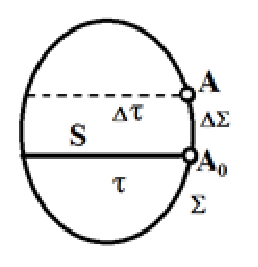
\includegraphics[width=0.2 \linewidth]{ger_1.eps}

{Рис. 1. Загальний вигляд області, яку займає рідина}
\end{center}

\vspace{+0,2cm}

Для довільної точки $A$ ця вимога може бути записана у вигляді розкладу у ряд Тейлора
\begin{eqnarray*}
   &&\frac{\partial \varphi}{\partial n}\bigg |_A = \frac{\partial \varphi}{\partial n}\bigg |_{A_0} +
       \xi \frac{\partial^2 \varphi}{\partial n \partial \tau_1}\bigg |_{A_0}+
       \frac{1}{2}\xi^2 \frac{\partial^3 \varphi}{\partial n \partial \tau_1^2}\bigg |_{A_0}+ \ldots =0.
\end{eqnarray*}
Тут через $\tau_1$ позначено вектор дотичного напрямку. Через довільність збурень вільної поверхні  $\xi$ в точці $A_0$ має виконуватися вимога
\begin{eqnarray*}
    &&\frac{\partial^k \varphi}{\partial n \partial \tau_1^{k-1}}\bigg |_{A_0} =0 \ \ \mbox{для} \ \ k=1,2, \ldots
\end{eqnarray*}


Дослідження показують, що нормальні похідні в точці $A_0$ у випадку нециліндричних резервуарів взагалі не існують через те, що точка $A_0$ є сингулярною. З другого боку не можна накладати на розв'язки крайової задачі другого порядку додаткові умови порядку вищого або рівного за порядок основного рівняння, тобто умови порядку вище одиниці є некоректними. В підсумку це свідчить про те, що не можна використовувати розв'язки задачі про власні частоти та форми коливань як координатних функцій при розв'язанні нелінійної задачі, а також не можна накладати якісь додаткові обмеження на задачу про вільні коливання рідини з метою виконання граничної умови неперетікання на продовженні бічної поверхні резервуара, куди можуть досягати гребні хвиль.

В роботах Н.~Є.~Жуковського було показано \cite{Zhu}, якщо рідина з рівнем заповнення до точки $A$ виконує коливання, то область рідини до рівня $A_0$ виконує такі ж самі рухи (в кінематичному сенсі) як і рідина в резервуарі з об'ємом заповнення до рівня $A_0$. Тобто додана частина рідини на кінематику руху вихідної рідини (характер течії) не чинить вплив за виключенням частот коливань. Тому було запропоновано метод допоміжної області \cite{Limgeo} для визначення координатних функцій для розв'язання нелінійної задачі про коливання рідини з вільною поверхнею, які задовільняють граничній умові неперетікання на стінках резервуара вище рівня незбуреної вільної поверхні, куди можуть досягати гребні хвиль. Ідея методу полягає в тому, що розв'язується задача про вільні коливання рідини для області рідини із заповненням до точки $A$, далі за координатні функції для області $\tau$ беруться визначені координатні функції, які задовільняють умові неперетікання на поверхні  $\Sigma_0+\Delta \Sigma$, а за координатні функції на вільній поверхні рідини $S_0$  беруться функції, які одержуються на горизонтальному перерізі, що проходить через точку  $A_0$. За своїм характером метод є наближеним, проте він враховує аналітичну природу розв'язку задачі про вільні коливання рідини і її сингулярні властивості. Успішність подальшого використання методу в основному визначається тим, що контур із сингулярними властивостями фактично переноситься від рівня, який відповідає положенню точки $A_0$ на рівень точки $A$, куди рідина вже взагалі не досягає. Таке винесення сингулярних точок за межі області рідини $\tau$ є типовим в інших задачах механіки ідеальної рідини. Практичне використання такого підходу для побудови координатних функцій для представлення розв'язків нелінійної задачі динаміки рідини в різних резервуарах нециліндричної форми (конус, сфера, гіперболоїд, еліпсоїд, параболоїд \cite{Kon,Limgeo}) дозволило досягнути відносної точності задовільнення граничної умови на $\Sigma_0$ порядку $10^{-5}$ і $10^{-3}$ на поверхні $\Delta \Sigma$, що більше ніж в 100 разів краще ніж для функцій, визначених за класичним методом. В підсумку це дозволяє з високою точністю задовільнити умовам розв'язуваності нелінійної задачі про рух рідини з вільною поверхнею \eqref{4} і підвищує точність задовільнення законів збереження енергії та маси, а також стійкість обчислювальних процедур.

Після використання розв'язків задачі на власні коливання рідини в резервуарі доповненої методом допоміжної області лишаються не задовільненими кінематична гранична умова на вільній поверхні та вимога збереження об'єму рідини у збуреному русі. Згідно з \cite{Limgeo} приймемо такі представлення шуканих розв'язків, які для цієї задачі є фактично формою пошуку розв'язку за методом Канторовича. Крім того, через те, що резервуар є тілом обертання надалі можливе відокремлення кутової координати у представленні форми пошуку розв'язку.
\begin{eqnarray}\label{7}
    &&\hskip-12mm \xi=\bar \xi (t)+\sum_i a_i(t) \bar \psi_i (\alpha) T_i(\theta); \ \ \ \varphi=\sum_i b_i(t)\psi_i(\alpha, \beta) T_i(\theta),
\end{eqnarray}
 де $\displaystyle \bar \psi_i (\alpha)=\frac{\partial \psi}{\partial z}\bigg |_{\beta=0} = \bigg ( \frac{1}{H}\frac{\partial \psi_i}{\partial \beta} - \frac{\alpha f'}{f} \frac{\partial \psi_i}{\partial \alpha}  \bigg ) \bigg |_{\beta=0}$. Також введено позначення $\bar \xi (t)$ -- функція, яка забезпечує виконання закону збереження об'єму рідини у її збуреному русі і обумовлена нециліндричністю області $\tau$, $\bar \psi_i(\alpha) T_i(\theta)$ -- форма коливань вільної поверхні рідини, $\psi_i (\alpha, \beta) T_i(\theta)$ -- потенціал швидкості, що відповідає руху рідини за цією формою. В представленні розв'язку \eqref{7} $a_i(t)$ і $b_i(t)$ є відповідно амплітудними параметрами збудження коливань вільної поверхні рідини та потенціалу швидкостей, що відповідають $i$-й формі коливань.

 Згідно з теоремою, що безвихровий рух ідеальної однорідної нестисливої рідини повністю визначається рухом її границь, змінні $a_i$ разом з параметрами руху резервуара $\vec \varepsilon$ є незалежними параметрами, які визначають рух границь області, а змінні $b_i$ і $\bar \xi$ є залежними. Покажемо як виконується виключення цих залежних змінних з кінематичних обмежень, а саме з вимоги збереження об'єму рідини та кінематичної граничної умови на вільній поверхні рідини. Зауважимо також, що саме ці дві вимоги формулюються через нелінійні співвідношення і для їхнього виконання будуть застосовані асимптотичні методи нелінійної механіки з припущенням про малість збурень вільної поверхні рідини $\xi$.

Величина $\bar \xi$ визначається з вимоги збереження об'єму рідини у її збуреному русі. З використанням розкладу значення інтеграла зі змінною верхньою границею в ряд по $\xi$ в околі $\xi=0$  одержимо з точністю до величин третього порядку малості (праворуч всі функції $f$ і їх похідні беруться для $\beta =0$).

\begin{eqnarray*}
    &&\Delta V =\int \limits_0^{2\pi} \int \limits_0^1 \left [ \int \limits_0^{\xi/H} [f(H\beta)]^2 d\beta  \right ] \alpha H d\alpha \theta=\\
    &&\int \limits_0^{2\pi} \int \limits_0^1 \left [f^2 \frac{\xi}{H} +ff'\frac{\xi^2}{H^2}+(f'^2 +ff") \frac{\xi^3}{3H^3}+ \ldots \right ] \alpha H d\alpha \theta.
\end{eqnarray*}

Якщо представити $\bar \xi$ у вигляді розкладу за ступенями малості збурення вільної поверхні рідини $\xi$, $\bar \xi = \bar \xi_1 +\bar \xi_2 + \bar \xi_3 +\bar \xi_4 $ (нижній індекс відповідає порядку малості величини відносно значення $\xi$), то одержимо (величини з верхнім індексом ''$v$'' є інтегралами від форм коливань, вираз для яких тут не приводяться)
\begin{eqnarray}\label{8}
    &&\hskip-8mm\bar \xi_1=0; \ \ \ \bar \xi_2=-\frac{f'}{\pi f} \sum_{i,j} a_i a_j \beta_{ij}^v; \ \ \ \\
    &&\hskip-8mm \bar \xi_3=-\frac{f'^2+ff"}{3\pi f^2} \sum_{i,j,k} a_i a_j a_k \gamma_{ijk}^v, \ldots \nonumber
\end{eqnarray}

Тепер після знаходження залежності $\bar \xi$ від $a_i$ представлення розв'язку задачі \eqref{7} задовільняє вимозі збереження об'єму рідини з точністю до величин третього порядку малості відносно $\xi$.

Для визначення залежності $b_i$ від $a_i$ скористаємося методом Гальоркіна. Введемо до розгляду диференціальний оператор
\begin{eqnarray*}
    &&\hskip-12mm L^*(\xi, \varphi) = \displaystyle \frac{\partial \xi}{\partial t} +\frac{1}{f^2} \frac{\partial \xi}{\partial \alpha} \frac{\partial \varphi }{\partial \alpha} +\frac{1}{\alpha^2 f^2} \frac{\partial \xi}{\partial \theta} \frac{\partial \varphi }{\partial \theta}-\frac{\alpha f'}{f} \frac{\partial \xi}{\partial \alpha} \frac{\partial \varphi }{\partial z} - \frac{\partial \varphi }{\partial z}=0.
\end{eqnarray*}
Виходячи з того, що система функцій $\bar \psi_k$ є формами коливань вільної поверхні, а значить вони є повною системою функцій, скалярні добутки нев'язок визначимо за схемою
\begin{eqnarray*}
     &&\int \limits_{S_0} L^*(\xi, \varphi) \big |_S \bar \psi_k dS=0, \ \ \ k=1, 2, \ldots ,
\end{eqnarray*}
при цьому диференціальний оператор $L^*$ розкладається в ряд за ступенями  $\xi$, що еквівалентно його проєктуванню на незбурену вільну поверхню $S_0$. Після підставлення розкладів шуканих невідомих \eqref{7} одержимо наступні вирази для залежності величин $b_i$ від $a_i$
\begin{eqnarray}\label{9}
    &&b_p^{(1)}=\sum_i \dot a_i\beta_{ip}^0; \ b_p^{(2)}=\sum_{i.j} \dot a_i a_j\gamma_{ijp}^0;\\
    &&\  b_p^{(3)}=\sum_{i.j,k} \dot a_i a_j a_k \delta_{ijkp}^0; \
         b_p^{(4)}=\sum_{i.j,k,l} \dot a_i a_j a_k a_l h_{ijklp}^0.\nonumber
\end{eqnarray}

У співвідношення \eqref{9} входять коефіцієнти, що визначаються через квадратури від функцій $\bar \psi_k$ і $\psi_k$  по незбуреній вільній поверхні. Після визначення залежностей \eqref{8} і \eqref{9} параметри $a_k$  можна вважати повною незалежною системою змінних, що характеризують рух обмеженого об'єму рідини (у випадку рухомого резервуара треба до цих параметрів ще додати параметри руху тіла-носія). Ці залежності встановлені аналітично (у квадратурах) для довільної кількості форм коливань до розв'язання варіаційної задачі. Тепер розклади шуканих змінних \eqref{7}, доповнені співвідношеннями \eqref{8} і \eqref{9}, відповідають вільній механічній системі, рух якої визначається незалежними параметрами $a_k$, що характеризують рух вільної поверхні рідини та  параметрам $\vec \varepsilon$, що характеризують рух тіла-носія.

Оскільки основною метою цієї роботи є викладення розширених можливостей варіаційних методів механіки, які ефективно працюють після належного аналізу всіх кінематичних обмежень задачі та виключенні цих обмежень до реалізації варіаційного принципу, викладення аналізу кінематичних обмежень задачі виконано докладно, а безпосередню реалізацію варіаційного принципу Гамільтона -- Остроградського ми не будемо викладати детально. Це викликано тим, що після побудови розкладів змінних (7), які через вибір координатних функцій і виключення залежних параметрів на основі співвідношень \eqref{8} і \eqref{9}, система, що досліджується, вже стає вільною і багато технічних проблем зникають.

Побудовані розклади \eqref{7} можна безпосередньо підставляти у функцію Лагранжа і при цьому система параметрів $a_k$ і $\varepsilon_i$ відповідає кількості ступенів вільності системи в рамках прийнятої моделі та за кількістю змінних є мінімальною.
Схема побудови дискретної моделі складається з двох етапів перетворення функції Лагранжа
\begin{eqnarray*}
    &&L(\xi, \varphi, \dot {\vec \varepsilon}) \rightarrow L(a_i, b_j, \bar \xi, \dot {\vec \varepsilon})\rightarrow L(a_i, \dot a_j, \dot {\vec \varepsilon}).
\end{eqnarray*}
Така схема ілюструє перехід спочатку від зв'язаної континуальної системи до зв'язаної дискретної системи, а потім, виключаючи кінематичні граничні умови на вільній поверхні та умову збереження об'єму рідини у її збуреному русі, здійснюється перехід до функції Лагранжа, що відповідає вільній системі з  числом параметрів, яке дорівнює числу ступенів вільності системи.

Для переходу від континуальної структури моделі тіло -- рідина до дискретної моделі можна застосувати метод Канторовича до варіаційного формулювання задачі, отриманого на основі принципу Гамільтона -- Остроградського. Просторове і поверхневе інтегрування у функції Лагранжа проводиться в змінних $\alpha, \theta, \beta$. В підінтегральному виразі відбувається диференціювання по $\beta$  членів, що містять потенціал швидкостей $\varphi$, і добутків цих членів на якобіан переходу від декартової геометрії до недекартової параметризації області $\tau_0$, яку займає рідина в незбуреному стані. Для порожнини обертання в цілому відмінності від випадку резервуарів циліндричної форми полягають в тому, що, по-перше, функції, за якими відбувається розклад потенціалу швидкостей, задовільняють умови неперетікання на змочуваних границях наближено, по-друге, додається умова збереження об'єму рідини у її збуреному русі, і, по-третє, при виконанні знесення на незбурену вільну поверхню рідини за допомогою ряду Тейлора окремих членів функції Лагранжа, кінематичної граничної умови на вільній поверхні і умови збереження об'єму рідини у її збуреному русі у порівнянні з випадком циліндричної області додаються геометричні нелінійності обумовлені переходом до недекартової параметризації області, яку займає рідина; вчетверте, слід забезпечити, щоб координатні функції задовільняли умові неперетікання на бічній поверхні рідини не лише для поверхні контакту у незбуреному стані $\Sigma_0$, а і на її певному продовженні над рівнем незбуреної вільної поверхні куди можуть досягати гребні хвиль $\Delta \Sigma$.

В результаті застосування даної методики можна отримати рівняння Лагранжа другого роду --  рівняння сумісного руху системи ''резервуар-рідина'' в амплітудних параметрах руху рідини з вільною поверхнею $a_k$ та параметрах руху тіла-носія ${\vec \varepsilon}$
\begin{eqnarray}\label{10}
    &&\hskip-12mm\sum_{k=1}^N p_{kr}(a_i,\dot a_j) \ddot a_k +\sum_{k=N+1}^{N+3} p_{kr} (a_i,\dot a_j) \ddot {\varepsilon}_{k-N}=q_r(a_i, \dot a_j, \varepsilon_l, \dot \varepsilon_m).
\end{eqnarray}
Через те, що другі похідні в ці рівняння входять лінійно, система звичайних диференціальних рівнянь легко приводиться до форми Коші, що сприяє подальшому аналітичному і чисельному дослідженню задачі. Легко показується, що породжувальна система диференціальних рівнянь є невиродженою, розподіл частот є відомим і діапазон розташування частот є компактним, що практично виключає проблеми прояву ефекту жорсткості при чисельному інтегруванні системи \eqref{10}.

%%%%%%%%%%%%%%%%%%%%%%%%%%%%%


\section{Вібраційне збудження руху системи резервуар-рідина в режимі сумісного руху}
Як приклад ефективної побудови моделі про сумісний рух резервуара і рідини з вільною поверхнею на основі методів аналітичної механіки континуальних систем розглянемо випадок резервуара у формі еліпсоїду обертання, маса якого $M_r=0,2 M_l$ (прояв рухомості рідини на рух резервуара буде суттєвим). Розглянуто випадок еліпсоїдального резервуара з півосями $a=1$ і $b=2$; випадок   відповідає розтягненому по вертикалі еліпсоїда з глибиною заповнення $H=0,75$. Резервуар здійснює рух в горизонтальній площині зі стану спокою під дією сили $F_x = A(M_r+M_l) \cos \omega t$ ($A$ -- множник, який для різних режимів підбирався так, щоб система виходила на режим нелінійних коливань, коли збурення на вільній поверхні мають порядок 0,2 від радіуса вільної поверхні рідини). Аналізувалися такі випадки зміни частот  $\omega=k_\omega \omega_c$, де $k_\omega=0,9; 0,98; 1,0; 1,02; 1,1; 1,5$, а $\omega_c$ -- частота сумісних коливань системи резервуар-рідина за першою формою. На рис.~2 представлені результати розрахунків зміни в часі збурень вільної поверхні рідини на бічній поверхні резервуара в площині $zOx$, в якій відбуваються коливання.

На рисунку зліва вгорі приведено глибину заповнення, згори в центі -- значення відносної частоти та амплітудного параметра збудження коливань системи. Звернемо увагу на те, що для частот суттєво менших за резонансні коливання вільної поверхні значно відрізняються від синусоїдального закону і спостерігається дрейф середнього значення. При наближенні до резонансної частоти спостерігається висока чутливість системи до амплітуди збудження і навіть до зміни частоти на декілька процентів. В характері розвинення коливань суттєво проявляється модуляція, при цьому частота зміни кривої модуляції спочатку зменшується і є найменшою для відносної частоти 0,98, а потім знову наростає. Це свідчить про те, що нелінійності в такій системі є м'якого типу.

%\vspace{-0,1cm}

\hspace{-1.85cm}
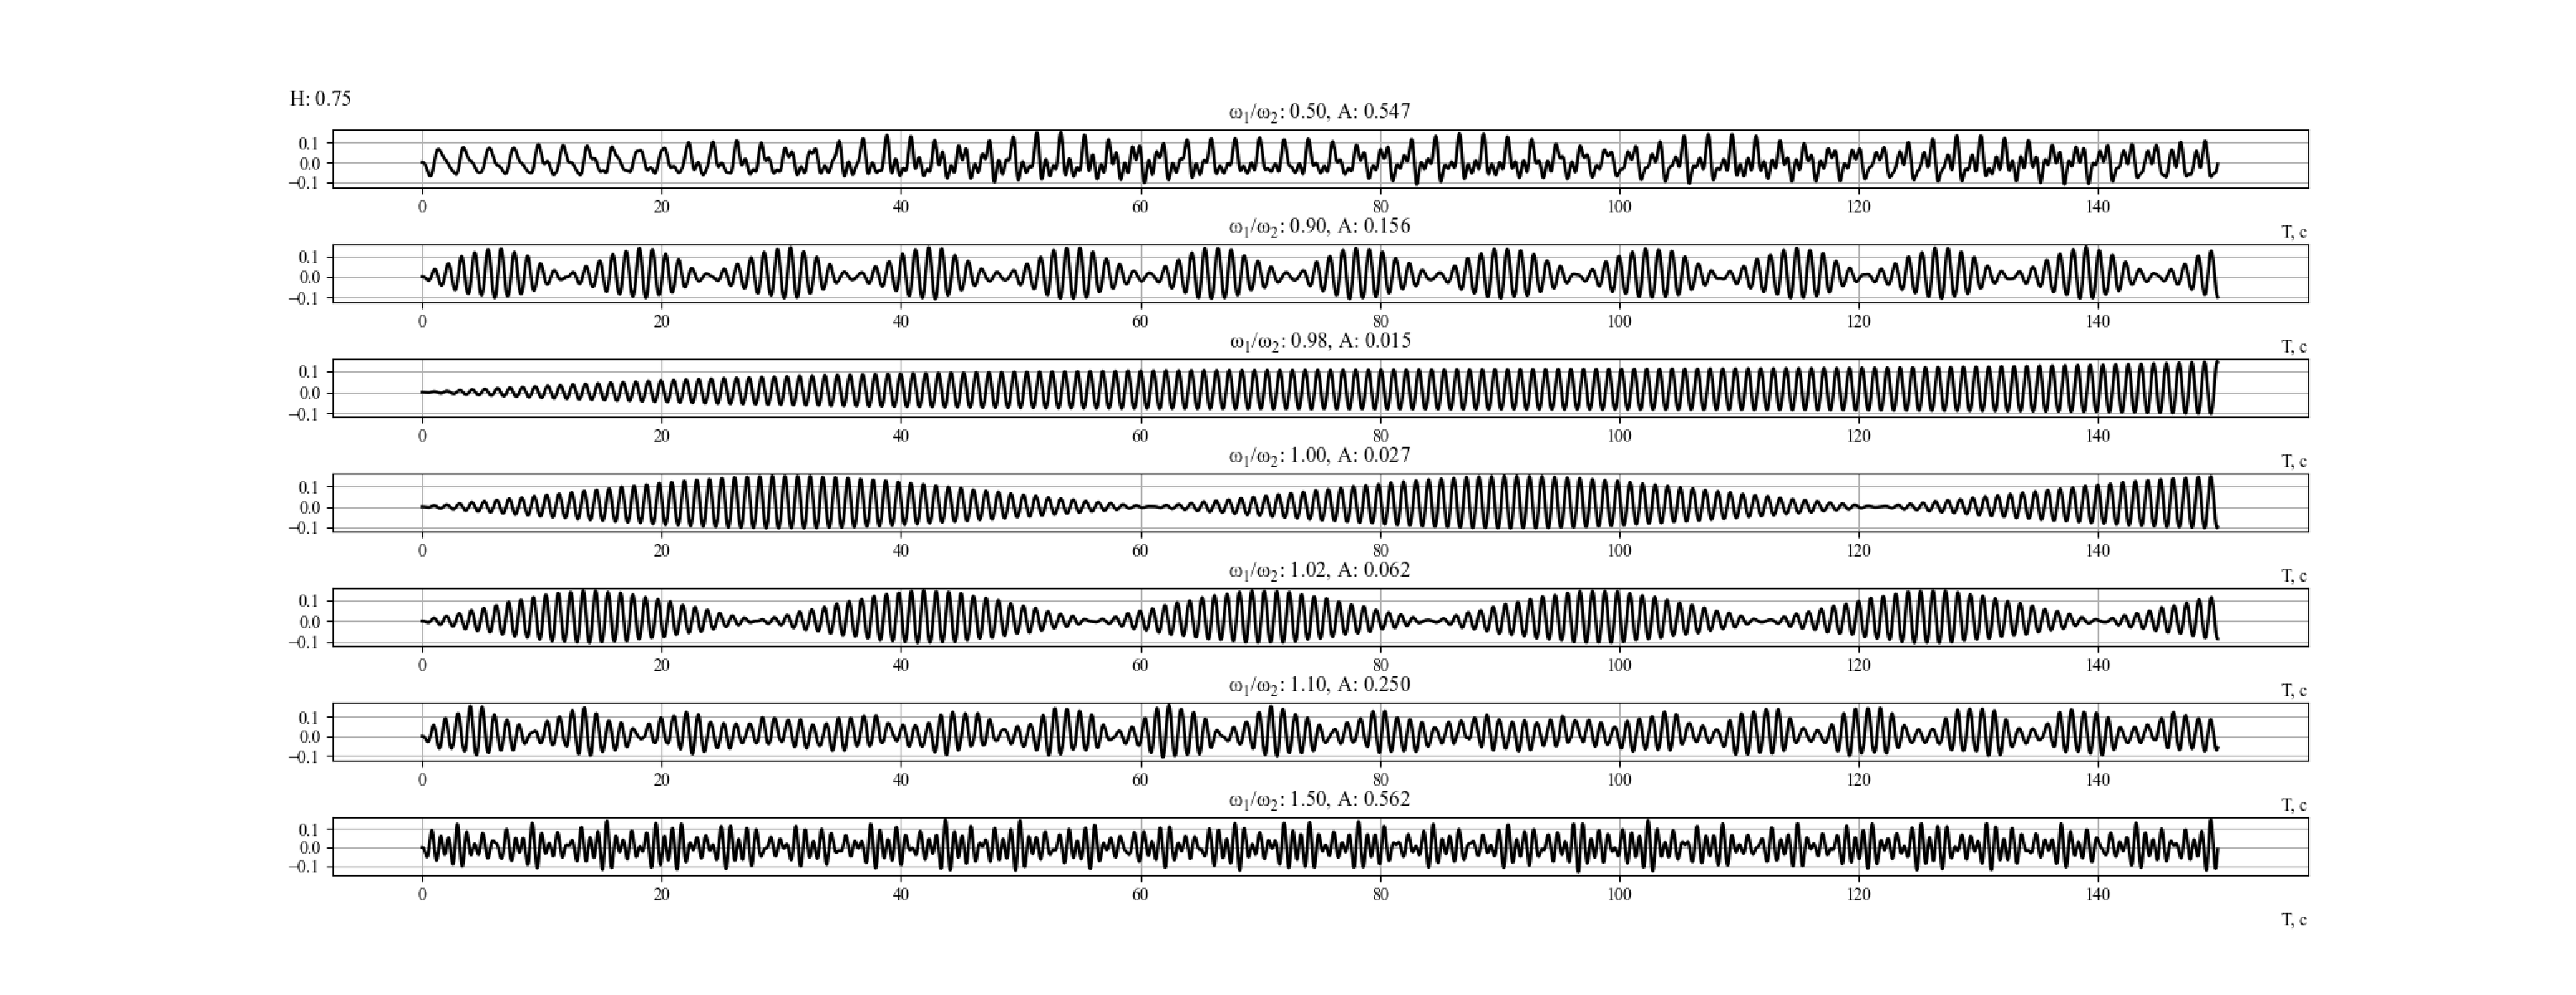
\includegraphics[width=1.22\linewidth]{ger_2.eps}

\vspace{-0,4cm}
\begin{center}
{Рис. 2. Збурення вільної поверхні рідини в різних частотних діапазонах}
\end{center}

\vspace{+0,2cm}

Вихід системи на режим усталених коливань не спостерігався, проте для відносної частоти 0,98 період модуляційної кривої є достатньо великим і в окремих роботах це помилково сприймалося як вихід на усталений режим коливань. Відмітимо також, що для відносної частоти 1 суттєво проявляється відмічений в експериментах режим антирезонанса, коли протягом декількох періодів коливання на вільній поверхні фактично зникають (їх амплітуда коливань є незначною), що помітно в околі часу приблизно 60 с і 120 с. Лінійна теорія прогнозує подібність поведінки системи через наближений збіг частот модуляції для значень відносних частот симетричних відносно власної частоти \cite{Sha}. Але в нашому випадку для частот 0,9 і 1,1 це не спостерігається, що пов'язане із виходом на режим, коли при формуванні модуляції беруть участь не дві форми коливань, а більше. Додаткові нелінійні властивості поведінки системи визначаються через трансцендентну залежність частот від номера форми, відміченого в \cite{Ono} і відповідного  ущільнення спектра коливань. Це обумовлює відсутність усталених режимів коливань.

Було розв'язано групу задач для різних варіантів еліпсоїдів і рівнів їх заповнення. Аналізуючи в комплексі одержані результати слід зазначити, що, по-перше, система резервуар-рідина демонструє високу чутливість до зміни частот особливо в безпосередньому околі резонансу. По-друге, значною мірою при однакових відносних амплітудах збурень вільної поверхні рідини прояв нелінійності визначається нахилом стінок в околі незбуреної вільної поверхні. Так для малих глибин і для випадків стисненої форми еліпсоїда нахил стінки резервуара в околі вільної поверхні значно відрізняється від вертикальних стінок. Це сприяє підсиленню прояву нелінійного характеру коливань, оскільки наближення нахилу стінок резервуара до вертикального положення призводить до зростання обмежень на рух рідини, і, до того ж до зростання частот і відстаней між ними. Це зменшує взаємовплив форм коливань, а значить спрощує характер розвинення коливань. По-третє, вагомо проявляється комплекс нелінійних ефектів розвинення коливань, а саме дрейф середнього значення коливань на низьких частотах, модуляція коливань, втрата регулярності коливань на високих частотах, антирезонанс, перевершення висоти горба хвилі над її впадиною. В-четверте, на всіх режимах вихід системи резервуар-рідина на режим усталених коливань не спостерігався. Одержані результати узгоджуються з відомими теоретичними та експериментальними даними \cite{Pal}.


\section{Висновки}
У роботі викладено оригінальні ідеї використання розширених можливостей аналітичної механіки суцільного середовища, зародження яких, судячи з усього, відбулося в рамках наукової школи Д.~О.~Ґраве і пізніше наукової школи М.~О.~Кільчевського. Ці ідеї є основою поглибленого аналізу постановки задач механіки суцільних середовищ і сприяють розвиненню конструктивних методів, створених на основі аналітичної механіки. Відмічені переваги і оригінальність цих підходів проілюстровано на задачі про нелінійні коливання рідини з вільною поверхнею, яку розглянуто в рамках нелінійної задачі динаміки сумісного руху системи, включаючи випадок резервуара нециліндричної форми.



%---------------  bibliography

\bibliographystyle{plainurl}
\bibliography{Lim_23}



%%%%%%%%%%%%%%%%%%%%%%%%%%%%%%%%%%%%%%%%%%%%%%%%%
%!!!!!! do not change this line - it will print the correct number of the last page
\printArticleAuthorsInfo{\thearticlesnum}
\label{last_page:\thearticlesnum}
%%%%%%%%%%%%%%%%%%%%%%%%%%%%%%%%%%%%%%%%%%%%%%%%%

\end{document}





\renewcommand{\refname}{Література}
\begin{thebibliography}{99}
\bibitem{Gan} {\it Гантмахер Ф.Р.} Лекции по аналитической механике. --- М.: Физматлит:~2005. --- 264 с.

\bibitem{Zhu} {\it Жуковсий Н.Е.} О движении твердого тела, имеющего полости, наполненные однородной капельной жидкостью. --- М.: Физматлит:~2005. --- 137~с.

\bibitem{Kan} {\it
Канторович Л.В., Крылов В.И.} Приближенные методы высшего анализа. --- Л. -- М.: Физматгиз:~1962. --- 708 с.

\bibitem{Koz} {\it
Коздоба Л.А.} Методы решения нелинейных задач теплопроводности. --- М.: Наука,~1975. --- 227 с

\bibitem {Limbo}
{\it Лимарченко О.С., Ясинский В.В.} Нелинейная динамика конструкций с жидкостью. --- К.: НТТУ КПИ,~1997. --- 338~с.

\bibitem{Pol} {\it Полак Л.С.} Вариационные принципы механики. --- С. П.,~1885. --- 930 с.

\bibitem{Kon} {\it Konstantinov A.V., Limarchenko O.S., Mel'nik V.N., Semenova I.Yu.} Problem of the parametric oscillations of a noncylindrical tank partially filled with a fluid // Int. Appl. Mechanics. --- 2016. --- Vol. 52, No. 6. --- P. 599-604

\bibitem{Lkib}
{\it Konstantinov A.V., Limarchenko V.O., Limarchenko O.S.} Motion control for structure with liquid based on compensation of the liquid hydrodynamic response // J Automation and Information Sci. --- 2020. --- Vol. 52, No. 6. --- P. 58-70


\bibitem{Limgeo} {\it Limarchenko O.S.} Specific features of application of perturbation techniques in problems of nonlinear oscillations of a liquid with free surface in cavities of noncylindrical shape // Ukrainian Math. J. --- 2007. --- Vol. 59, No. 1. --- P. 46-69.

\bibitem{LS}
{\it Limarchenko O.S., Semenovich K.O.} Energy redistribution between the reservoir and liquid with free surface for angular motions of the system // J. Mathem. Sci. --- 2017. --- Vol.~222, N.~3. --- P. 296-303.


\bibitem{Ono}
{\it Onorato M., Vozella L., Proment D., Lvov V.} Route to thermalization in the Fermi-Pasta-Ulam system // PNAS. ---  2015. ---  Vol.~112,~No.~14.~--- P.~4208-4213.


\bibitem{Pal}
{\it Pal P.} Sloshing of liquid in partially filled container -- an experimental study // Int. J. Recent Trends in Engineering. --- 2009. --- Vol.~1,~No.~6. --- P.~1--5.

\bibitem{Sha} {\it Shaoa W., Yanga J., Hu Z, Tao L.} Coupled analysis of nonlinear sloshing and ship motions // Applied Ocean Research. --- 2015. --- 47. --- P. 85-97
\end{thebibliography}
